\subsection{Pitch Generation}\label{subsec:Pitch_Generation}

Die Hauptaufgabe der Komponente Pitch Generation ist es das Audiosignal aus dem Rechtecksignal der Tonhöhenantenne (Pitch Antenna) zu generieren. 


\begin{figure}[h!]
	\centering
	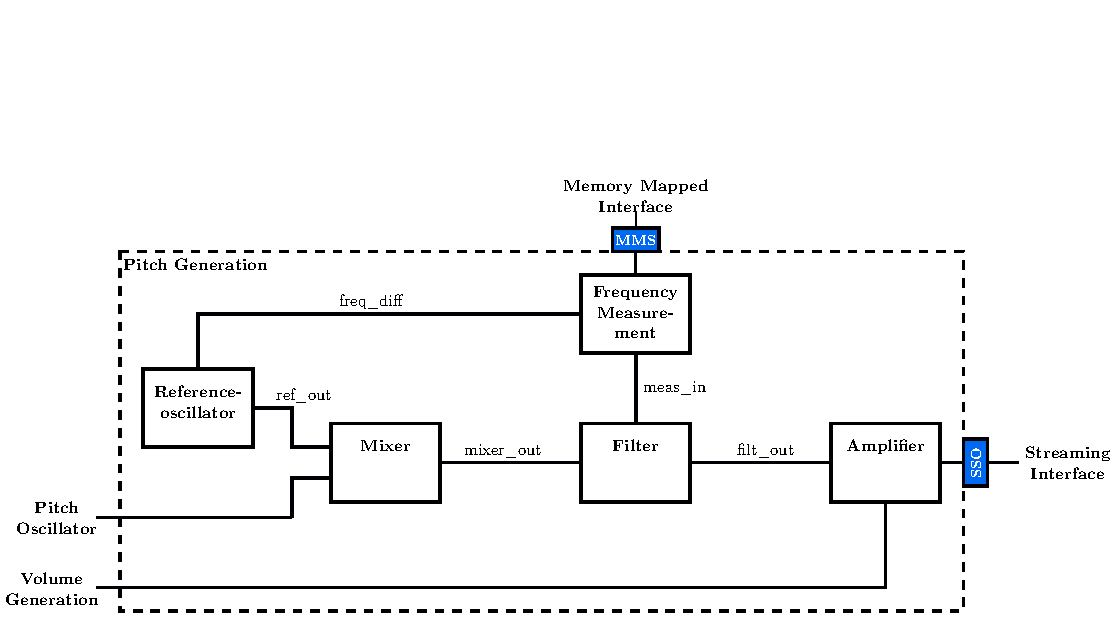
\includegraphics[width=1\textwidth]{Blockschaltbild_pitch.pdf}
	\caption{Blockschaltbild der Custom IP Pitch Generation} 
	\label{img:Blockschaltbild_pitch}
\end{figure}  



\paragraph{Referenzoszillator}

\begin{figure}[h!]
	\centering
	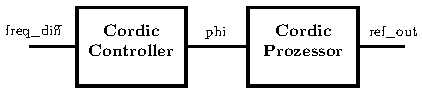
\includegraphics[width=0.53\textwidth]{Referenceoscillator.pdf}
	\caption{Aufbau des Referenzoszillators} 
	\label{img:Referenceoscillator}
\end{figure}  

\paragraph{Filter}

\begin{figure}[h!]
	\centering
	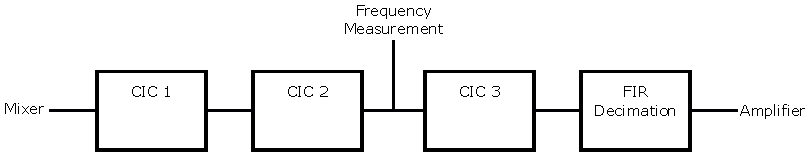
\includegraphics[width=1\textwidth]{Filter_pitch.pdf}
	\caption{Aufbau des Filters in der Komponente Pitch Generation} 
	\label{img:Filter_Pitch}
\end{figure}  

\paragraph{Frequenzmessung, Kalibration \& Glissandoeffekt}

\begin{figure}[h!]
	\centering
	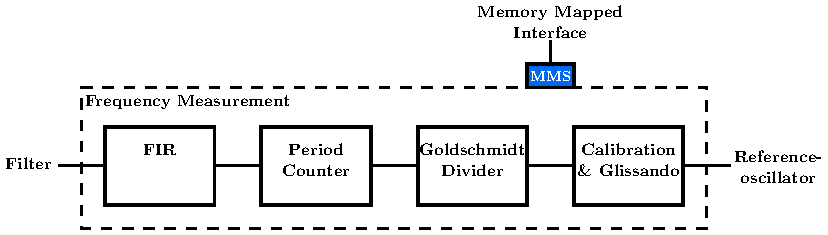
\includegraphics[width=1\textwidth]{freq_meas_pitch.pdf}
	\caption{Aufbau der Frequenzmessung, Kalibration und Glissandoeffekt in der Komponente Pitch Generation} 
	\label{img:freq_meas_pitch}
\end{figure}  